% Preamble. Don't worry about it.
\documentclass{article}
\usepackage{setspace,graphicx,fancyhdr}
\usepackage[utf8]{inputenc}
\usepackage[left=1in,top=1in,right=1in,bottom=1in]{geometry} % Document margins
\onehalfspacing

% For custom footers
\pagestyle{fancy}
\fancyhead{}                        % clear all header fields
\renewcommand{\headrulewidth}{0pt}  % no line in header area
\fancyfoot{}                        % clear all footer fields
\fancyfoot[LE,RO]{\thepage}         % for page #s
\fancyfoot[RE,LO]{
\includegraphics{../images/logo/markshark-1x}}

% Setting the depth for Table of Contents
\setcounter{tocdepth}{2}

\begin{document}

% --- TITLE PAGE ---
\title{Donnervögel Consulting \\ MarkShark Grading System \\ Design Document}
\author{\textbf{Phase Lead: Stephen Laboucane} \\ Markus Balaski \\ Ian Pun \\
  Graeme Smith \\ Jordan Toering \\  Colin Woodbury \\ Chazz Young}
\maketitle
\centerline{
\includegraphics{../images/logo/markshark-10x}}
\clearpage
% ------------------

% --- REVISION HISTORY ---
\textbf{Revision History}
\begin{center}
  \begin{tabular}{| c | c | c | l |}
    \hline
    Version & Date & Members & Changes\\
    \hline
    1.0 & 2014 Mar 14 (Fri) & Markus B. & Document created.\\
    & & Graeme S. & \\
    & & Jordan T. & \\
    & & Stephen L. & \\
    & & Ian P. & \\
    & & Colin W. & \\
    & & Chazz Y. & \\
    \hline
  \end{tabular}
\end{center}
\clearpage
% ------------------------

% --- TABLE OF CONTENTS ---
\tableofcontents
\clearpage
% -------------------------

\section{High Level Design}
\subsection{Architecture Diagram}
\centerline{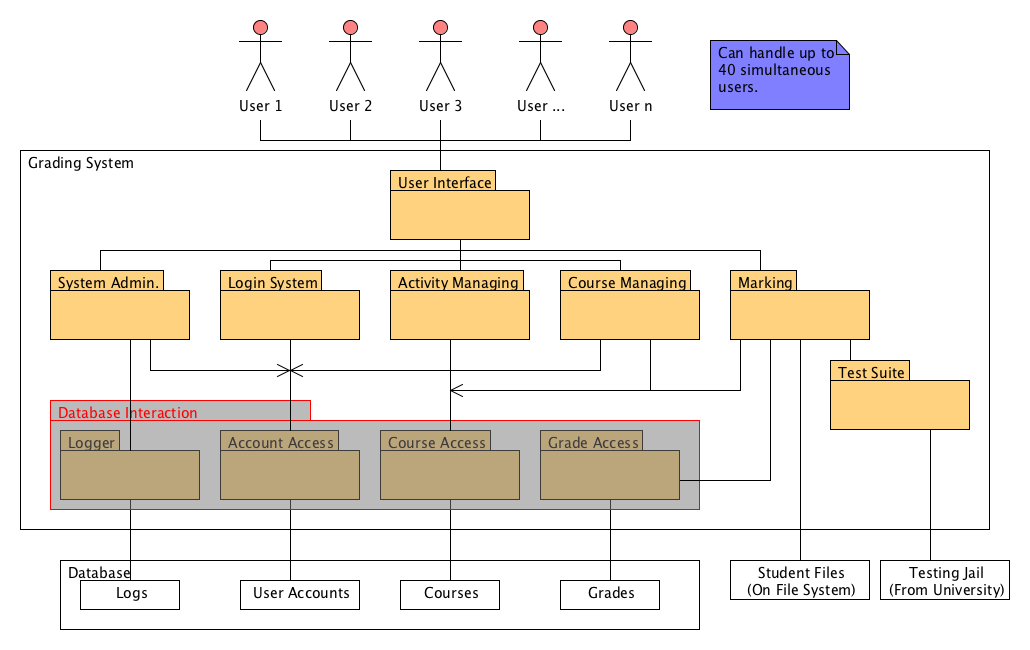
\includegraphics[scale=0.6]{../images/architectureDiagram}}

\subsection{Sub-system Descriptions}
\subsection{Refined Use Cases}
\textbf{Use Case Name: testCourse (\#3.9)}

\textbf{Scenario:}
TA Marker Joe Fresh runs the test suite to grade Student Tina Turner’s “Assignment 4” 
code.

\textbf{Preconditions:}
\begin{itemize}
	\item Joe has logged in successfully.
	\item Joe has navigated to the “Marking” page for Assignment 4. (\textbf{Marking 
		$\rightarrow$ Courses $\rightarrow$ Select Activity $\rightarrow$ Assignment 4}).
	\item The test suite  and database are ready to be initialised.
	\item Tina has turned in Assignment 4, and her code can be compiled.
\end{itemize}

\textbf{Main Flow of Events:}
\begin{enumerate} 
	\item Joe clicks on the “Test Code” button in the bottom right corner of the screen.
	\item The program will compile and run Tina’s  code.
	\item Assuming the code generates output, an output file is generated.
	\item The screen will change to the “Test Suite” page, displaying the output 
		generated code, the solution code and a diff (the differences between the 
		two documents) of the two outputs.
	\item Joe will look at the diff, then the solution code and mark the output by
		tabbing between the test suite and the rubric.	
	\item Additionally, Joe may comment on Tina’s code by 	clicking the “Submit 
		Comment” button.
	\item Joe finishes marking and clicks “Submit”.
\end{enumerate}

Textbf{Postconditions:}

\begin{itemize}
\item The program saves the grade to the database. 
\item Joe is returned to the “Select Activity” page for Assignment 4.
\end{itemize}

\textbf{Exceptional Flow of Events:}
\begin{enumerate}
 	\item If the compiled code doesn’t generate output, or crashes from a runtime 
 		error, then a message will appear in the “Student Solution” field saying that  
 		no output could be generated.
	\item If the rubric is not completely filled out (i.e. one or more of the items in the 
		rubric that do not have a mark)
\end{enumerate}

%INSERT COLLABORATION DIAGRAM HERE%
\section{Low Level Design}
\subsection{Interaction Diagrams}
\subsection{Class Diagram}

\section{Data Persistence}

\end{document}
